%%%%%%%%%%%%%%%%%%%%%%%%%%%%%%%%%%%%%%%%%
% The Legrand Orange Book
% LaTeX Template
% Version 2.1.1 (14/2/16)
%
% This template has been downloaded from:
% http://www.LaTeXTemplates.com
%
% Original author:
% Mathias Legrand (legrand.mathias@gmail.com) with modifications by:
% Vel (vel@latextemplates.com)
%
% License:
% CC BY-NC-SA 3.0 (http://creativecommons.org/licenses/by-nc-sa/3.0/)
%
% Compiling this template:
% This template uses biber for its bibliography and makeindex for its index.
% When you first open the template, compile it from the command line with the 
% commands below to make sure your LaTeX distribution is configured correctly:
%
% 1) pdflatex main
% 2) makeindex main.idx -s StyleInd.ist
% 3) biber main
% 4) pdflatex main x 2
%
% After this, when you wish to update the bibliography/index use the appropriate
% command above and make sure to compile with pdflatex several times 
% afterwards to propagate your changes to the document.
%
% This template also uses a number of packages which may need to be
% updated to the newest versions for the template to compile. It is strongly
% recommended you update your LaTeX distribution if you have any
% compilation errors.
%
% Important note:
% Chapter heading images should have a 2:1 width:height ratio,
% e.g. 920px width and 460px height.
%
%%%%%%%%%%%%%%%%%%%%%%%%%%%%%%%%%%%%%%%%%

%----------------------------------------------------------------------------------------
%	PACKAGES AND OTHER DOCUMENT CONFIGURATIONS
%----------------------------------------------------------------------------------------

\documentclass[11pt,fleqn]{book} % Default font size and left-justified equations

\usepackage{wasysym}
\usepackage{esint} % various fancy integral symbols
\usepackage{tikz}
\usepackage{tikz-3dplot}
\usepackage{pgfplots}
\pgfplotsset{compat=1.17}
\usepackage[french]{babel}

\usetikzlibrary {arrows.meta} 

\newcommand{\dd}{\mathrm{d}}
\newcommand{\div}{\mathrm{div}}
\newcommand{\rot}{\vv{\mathrm{div}}}
\newcommand{\grad}{\vv{\mathrm{grad}}}

\usepackage[d]{esvect}

\definecolor{myred}{RGB}{243,102,25}


%----------------------------------------------------------------------------------------
%SPECIFIC TIKZ COMMANDS

\usepackage{ifthen}
\usepackage{tikz,pgfplots}
\usepackage{tikz-3dplot}
\usepackage{auto-pst-pdf}
\usepackage{pst-plot}
\usepackage{pst-magneticfield}
\usepackage[outline]{contour} % glow around text
\usetikzlibrary{angles,quotes} % for pic (angle labels)
\usetikzlibrary{arrows,arrows.meta}
\usetikzlibrary{calc}
\usetikzlibrary{decorations.markings}
\tikzset{>=latex} % for LaTeX arrow head
\usepackage{xcolor}
\colorlet{Ecol}{myred!90!black}
\colorlet{EcolFL}{myred!80!black}
\colorlet{veccol}{white!45!black}
\colorlet{projcol}{blue!70!black}
\colorlet{EFcol}{myred!60!black}
\colorlet{Bcol}{myred!90}
\colorlet{BFcol}{myred!70!black}
\colorlet{veccol}{white!45!black}
\colorlet{Icol}{black}
\colorlet{Ampcol}{black}
\tikzstyle{BField}=[->,thick,Bcol]
\tikzstyle{current}=[->,Icol,thick]
\tikzstyle{force}=[->,thick,BFcol]
\tikzstyle{vector}=[->,thick,veccol]
\tikzstyle{velocity}=[->,very thick,vcol]
\tikzstyle{metal}=[top color=black!15,bottom color=black!25,middle color=black!20,shading angle=10]
\tikzstyle{darkmetal}=[top color=black!40,bottom color=black!70,middle color=black!30,shading angle=10]
\tikzstyle{lightmetal}=[thin,black!30,top color=black!10,bottom color=black!25,middle color=black!15,shading angle=10]
\tikzstyle{proj}=[projcol!80,line width=0.08] %very thin
\tikzstyle{area}=[draw=veccol,fill=veccol!80,fill opacity=0.6]
\tikzstyle{measline}=[{Latex[length=3]}-{Latex[length=3]}]
\tikzset{
  BFieldLine/.style={ultra thick,Bcol,decoration={markings,mark=at position #1 with {\arrow{latex}}},postaction={decorate}},
  BFieldLine/.default=0.5,
  Ampcurve/.style={ultra thick,Ampcol,decoration={markings,mark=at position #1 with {\arrow{latex}}},
                          postaction={decorate}},
  Ampcurve/.default=0.55,
  pics/Bin/.style={
    code={
      \def\R{0.12}
      \draw[pic actions,line width=0.6,#1,fill=white] % ,thick
        (0,0) circle (\R) (-135:.75*\R) -- (45:.75*\R) (-45:.75*\R) -- (135:.75*\R);
  }},
  pics/Bout/.style={
    code={
      \def\R{0.12}
      \draw[pic actions,line width=0.6,#1,fill=white] (0,0) circle (\R);
      \fill[pic actions,#1] (0,0) circle (0.3*\R);
  }},
  pics/Bin/.default=Bcol,
  pics/Bout/.default=Bcol,
}
\tikzstyle{measure}=[fill=white,midway,outer sep=2]
%\newcommand\arrmark[1]{mark=at position #1 with {\arrow{latex}}}
%\def\myarrmark#1{mark=at position #1 with {\arrow{latex}}}
\contourlength{1.4pt}

% RING SHADING
\makeatletter
\pgfdeclareradialshading[tikz@ball]{ring}{\pgfpoint{0cm}{0cm}}%
{rgb(0cm)=(1,1,1);
rgb(0.719cm)=(1,1,1);
color(0.72cm)=(tikz@ball);
rgb(0.9cm)=(1,1,1)}
\tikzoption{ring color}{\pgfutil@colorlet{tikz@ball}{#1}\def\tikz@shading{ring}\tikz@addmode{\tikz@mode@shadetrue}}
\makeatother



%-------------------------------------------------------------------


\input{structure} % Insert the commands.tex file which contains the majority of the structure behind the template

\begin{document}
%----------------------------------------------------------------------------------------
%	TITLE PAGE
%----------------------------------------------------------------------------------------

%\begingroup
%\thispagestyle{empty}
%\begin{tikzpicture}[remember picture,overlay]
%\coordinate [below=12cm] (midpoint) at (current page.north);
%\node at (current page.north west)
%{\begin{tikzpicture}[remember picture,overlay]
%\node[anchor=north west,inner sep=0pt] at (0,0) {
\includegraphics[width=\paperwidth]{background}}; % Background image
%\draw[anchor=north] (midpoint) node [fill=ocre!30!white,fill opacity=0.6,text opacity=1,inner sep=1cm]{\Huge\centering\bfseries\sffamily\parbox[c][][t]{\paperwidth}{\centering Cours de Physique-Chimie\\[15pt] % Book title
%{}\\[20pt] % Subtitle
%{\huge Lycée Baimbridge MP 2025-2026}}}; % Author name
%\end{tikzpicture}};
%\end{tikzpicture}
%\vfill
%\endgroup

%----------------------------------------------------------------------------------------
%	COPYRIGHT PAGE
%----------------------------------------------------------------------------------------

%\newpage
%~\vfill
%\thispagestyle{empty}

%\noindent Copyright \copyright\ CC BY 4.0 2025 Basile Poujol\\ % Copyright notice

%\noindent Licensed under the Creative Commons Attribution-NonCommercial 4.0 Unported License (the ``License''). You may not use this file except in compliance with the License. You may obtain a copy of the License at \url{http://creativecommons.org/licenses/by-nc/3.0}. See the License for the specific language governing permissions and limitations under the License.\\ % License information

%----------------------------------------------------------------------------------------
%	TABLE OF CONTENTS
%----------------------------------------------------------------------------------------

%\usechapterimagefalse % If you don't want to include a chapter image, use this to toggle images off - it can be enabled later with \usechapterimagetrue

\chapterimage{nasa_solar_magnetic_field.jpg} % Table of contents heading image

%\pagestyle{empty} % No headers

%\tableofcontents % Print the table of contents itself

%\cleardoublepage % Forces the first chapter to start on an odd page so it's on the right

%\pagestyle{fancy} % Print headers again



%\part{\'{E}lectromagnétisme}

\setcounter{chapter}{3}

\chapter{Magnétostatique}

Dans le chapitre précédent, nous nous sommes intéressés au champ électrique et à la façon dont il est créé par une distributions de charges en régime permanent. En particulier, nous avons vu que la distribution de charges détermine le champ électrique en tout point de l'espace, et que l'on peut utiliser le théorème de Gauss pour déterminer le champ si les symétries du problème sont suffisantes.

Dans ce chapitre, nous allons maintenant nous intéresser au champ magnétique, toujours en nous concentrant sur le régime stationnaire. Le champ magnétique n'est pas produit par la distribution de charges électriques, mais plutôt par les courants, comme cela a été démontré par {\O}rsted.

\begin{encart}[L'expérience d'{\O}rsted]
    Le danois Hans Christian {\O}rsted, en 1820, réalise une expérience très simple dont le résultat se répand rapidement dans toute la communauté scientifique. Il place un fil électrique près d'une boussole et montre que lorsque le fil est parcouru par un courant électrique, la boussole est déviée.

    Il montre ainsi que la circulation de courant électrique produit un champ magnétique. C'est le début de nombreuses autres expérimentations, menées notamment par Ampère.

    \begin{center}
    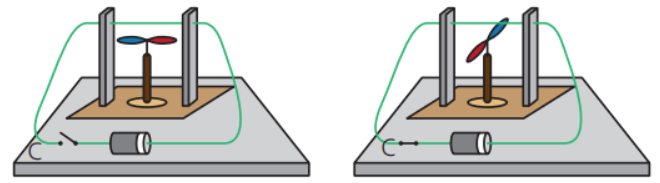
\includegraphics[width=0.7\textwidth]{Pictures/oersted_experiment.png} \\
    Schéma de l'expérience d'{\O}rsted. Lorsque le circuit électrique est fermé, l'aiguille de la boussole est déviée. Source : Planetajivo.
    \end{center}
\end{encart}

\section{Le courant électrique}

Nous allons donc nous intéresser plus spécifiquement au courant électrique.

\begin{definition}[Courant électrique]
    Le courant électrique $i$ à travers un fil est défini comme la quantité de charge qui traverse le fil par unité de temps à travers un point donné du fil :
    \begin{equation}
        i = \frac{\dd q}{\dd t}
    \end{equation}
    Il se mesure en Ampères (A).
    Un signe est attribué au courant, selon l'orientation choisie pour le fil.
\end{definition}

Quelle est l'interprétation microscopique du courant électrique ? Pour cela, nous devons regarder le fil de plus près. A cette échelle, le fil est un conducteur de taille finie, que l'on peut assimiler à un cylindre de rayon $R$.

Les métaux sont des éléments du tableau périodique qui peuvent perdre des électrons facilement et former des cations (métaux alcalins ou métaux de transition; cf cours de MPSI). Ainsi, ils forment un réseau cristallin de cations dans lequel se déplace un nuage électronique. 

\begin{figure}[htbp]
    \centering
    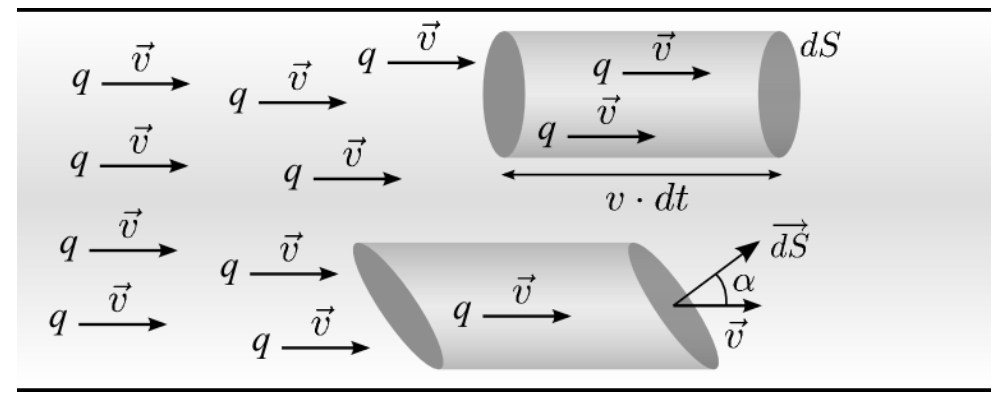
\includegraphics[width=0.7\linewidth]{Pictures/courant_electrique.png}
    \caption{Des électrons de charge $q = -e$ circulent dans un fil électrique avec la vitesse $\vv v$. Ce schéma montre le flux d'électrons à travers des éléments de surface dans le fil. Source : Poly de cours de Daniel Buskulic.}
    \label{fig:courant_electrique}
\end{figure}

Nous allons noter $\vv v$ la vitesse moyenne des électrons, et $n$ la densité moyenne d'électrons (en électrons par mètre cube). Les électrons portent une charge $q = -e$. 

\begin{capex}
Considérons un petit élément $\dd S$ de la section du fil pris perpendiculaire au mouvement des électrons, à la coordonnée $x$ (partie haute de la figure \ref{fig:courant_electrique}). Déterminer le nombre d'électrons qui traversent la surface $\vv{\dd S}$ pendant $\dd t$. En déduire le courant qui circule à travers la surface $\dd S$.
\end{capex}

% sont ceux qui se trouvaient à l'instant $t$ dans le volume $\dd V$ compris entre $x-v \dd t$ et $x$, de côté $\dd S$.
%On a :
%\begin{equation}
%\dd V = v \dd t \times \dd S
%\end{equation}
%Le nombre d'électrons qui traverse $\dd S$ pendant $\dd t$ est donc donné par :
%\begin{equation}
%    \dd N = n \times (v \dd t \times \dd S)
%\end{equation}
%ce qui correspond à une charge :
%\begin{equation}
%    \dd q = - n e v \dd S \dd t
%\end{equation}

De manière générale, on peut montrer que si l'élément de surface n'est pas pris perpendiculaire au mouvement des électrons (bas de la figure \ref{fig:courant_electrique}), l'expression reste inchangée avec un produit scalaire :
\begin{equation}
    \dd q = - n e \vv v \cdot \vv{\dd S} \dd t
\end{equation}

Cette interprétation microscopique nous amène à définir le vecteur densité de courant volumique :

\begin{definition}[Densité volumique de courant]
    La densité volumique de courant, notée $\vv j$, est définie telle que la quantité de charge traversant une surface élémentaire $\vv{\dd S}$ pendant une durée $\dd t$ soit donnée par :
    \begin{equation}
        \dd q = \vv j \cdot \vv{\dd S} \dd t
    \end{equation}
    Elle se mesure en A$\cdot$m$^{-2}$.
\end{definition}

Le calcul précédent nous fournit alors directement son expression :

\begin{proposition}
    Dans un métal conducteur, la densité volumique de courant $\vv j$ est reliée à la densité des électrons $n$ et leur vitesse $\vv v$ par :
    \begin{equation}
        \vv j = - n e \vv v
    \end{equation}
    De manière plus générale, dans un matériau contenant des porteurs de charges de charge $q_i$ avec une densité $n_i$ et une vitesse $\vv{v_i}$ on a :
    \begin{equation}
        \vv j  = \sum_i n_i q_i \vv{v_i}
    \end{equation}
\end{proposition}

Nous pouvons alors interpréter l'intensité totale du courant qui traverse le fil comme un flux du vecteur densité volumique de courant :

\begin{proposition}
    L'intensité $i$ qui traverse un fil de section $\Sigma$ est donnée par le flux de la densité volumique de courant à travers cette surface :
    \begin{equation}
        i = \iint_\Sigma \vv j \cdot \vv{\dd S}
    \end{equation}
\end{proposition}

\begin{demonstration}
    Nous notons $\Sigma$ la section du fil électrique. La charge totale qui traverse le fil pendant $\dd t$ est obtenue  en intégrant sur tous les éléments de surface formant la section du fil:
\begin{equation}
    \dd q_{tot} = \iint_\Sigma \dd q = \iint_\Sigma \vv j \cdot \vv{\dd S} \dd t
\end{equation}
d'où l'intensité qui traverse le fil :
\begin{equation}
    i = \frac{\dd q_{tot}}{\dd t} = \iint_\Sigma \vv j \cdot \vv{\dd S}
\end{equation}
\end{demonstration}

Nous avons ainsi pu, dans cette partie, apporter une définition rigoureuse du courant électrique ainsi qu'une mesure locale de ce courant électrique via la densité volumique de courant $\vv j$.

\section{Le champ magnétique}

\subsection{Action sur une particule chargée}

Nous allons maintenant décrire le champ magnétique. 
Le champ magnétique, à l'instar du champ électrique, n'est défini théoriquement. Il est défini par son action sur une particule chargée via la force de Lorentz :
\begin{proposition}[Force magnétique de Lorentz]
    Une particule chargée, de charge $q$ et de vitesse $\vv v$, placée dans un champ magnétique uniforme $\vv B$ subit une force magnétique :
    \begin{equation}
        \vv F = q \vv v \wedge \vv B
    \end{equation}
\end{proposition}

En pratique, cette force magnétique peut se superposer à la force électrique $\vv F = q \vv E$ qui agit en présence d'un champ électrique.

Le champ magnétique, de la même manière que le champ électrique, peut être visualisé à travers les lignes de champ. En particulier, en MPSI, nous avons vu l'allure des lignes de champ créées par un aimant.

Une propriété importante de la force magnétique de Lorentz est qu'elle est toujours perpendiculaire au mouvement si bien qu'elle ne travaille pas :
\begin{proposition}
    La composante magnétique de la force de Lorentz ne travaille pas.
\end{proposition}
En particulier, il n'est pas possible de tracer des "surfaces équipotentielles" pour visualiser le champ magnétique : de telles surfaces n'existent pas. 

La force magnétique ne modifie donc pas l'énergie cinétique des particules chargées, ainsi la norme de leur vitesse reste constante. Cependant, la force magnétique influence la direction du mouvement de ces particules : elle agit sur la composante de la vitesse perpendiculaire au champ magnétique $\vv{v}_\perp$, et a tendance à enrouler les trajectoires autour des lignes de champ, ce qui crée une trajectoire en hélice autour des lignes de champ. les particules chargées sont donc guidées par le champ magnétique.

\begin{figure}[htbp]
    \centering
    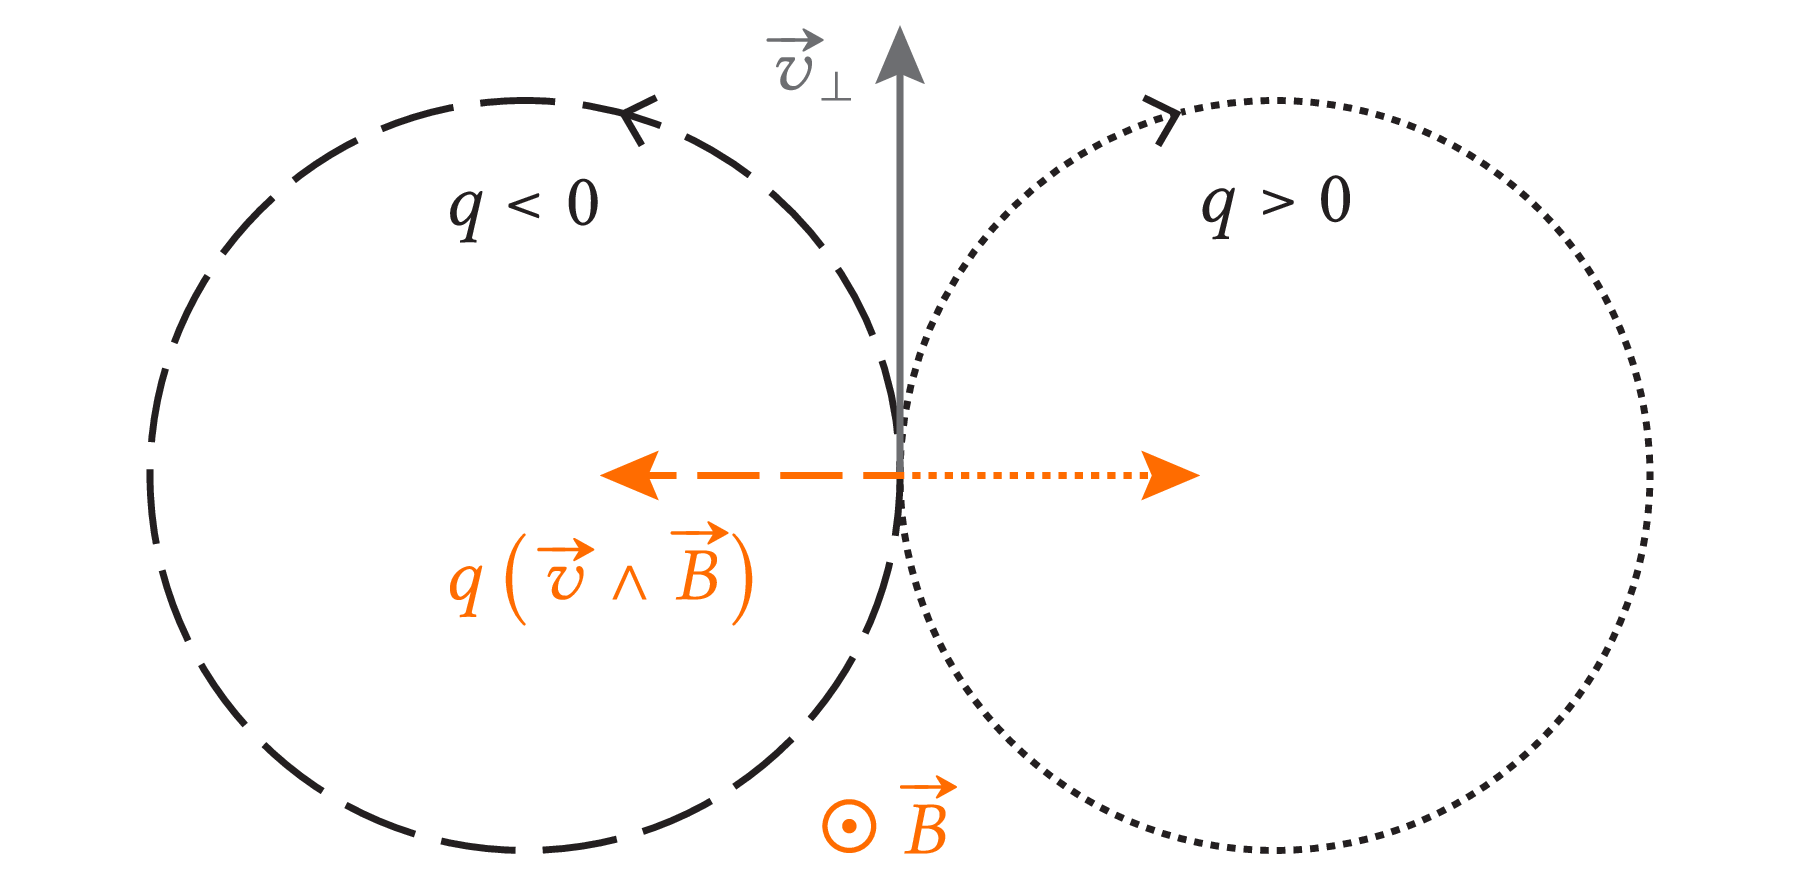
\includegraphics[height=0.3\linewidth]{Pictures/Figure_Chap5_1.png} 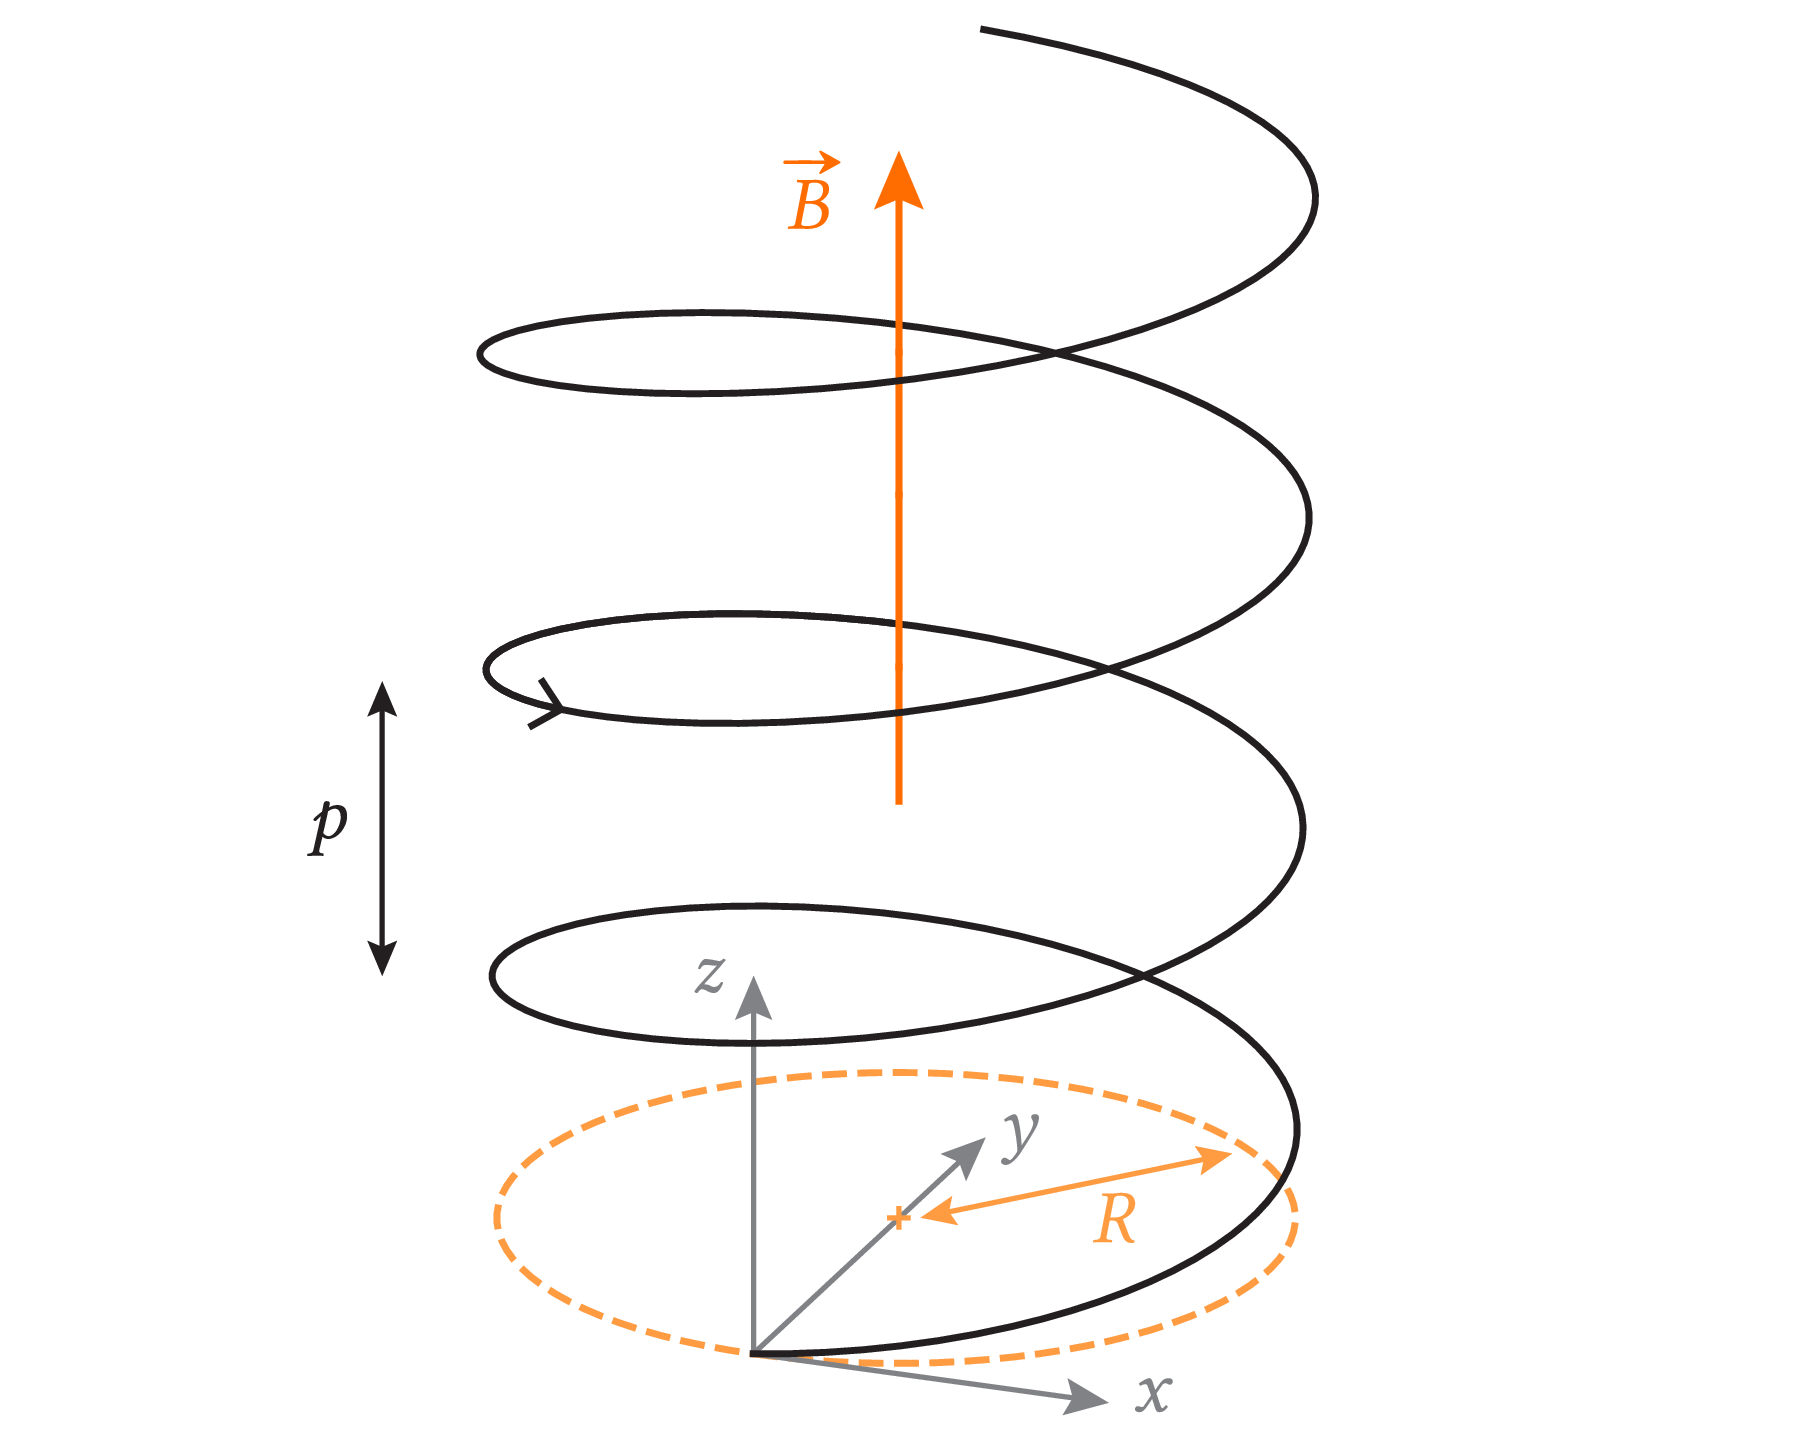
\includegraphics[height=0.3\linewidth]{Pictures/Figure_Chap5_2.png}
    \caption{Trajectoire d'une particule chargée dans un champ magnétique uniforme, projetée dans le plan perpendiculaire au champ magnétique (à gauche) ou vue en perspective (à droite). Source : Fillette, Froustey et Roussile (2023). \textit{Physique pour l'agrégation.}}
    \label{fig:trajectoires}
\end{figure}

Cette propriété est utilisée dans les accélérateurs de particules, mais elle joue aussi un rôle important dans des phénomènes naturels tels que les aurores polaires.

\begin{encart}[Les aurores polaires]
    Les aurores polaires sont des rideaux lumineux observés aux hautes latitudes. Ce phénomène a été compris grâce aux travaux de la scientifique américaine Joan Feynman. En 1977, en utilisant les données de la sonde Explorer 33 lancée par la NASA, elle a pu montrer que les aurores résultent d'une interaction entre des particules chargées émises par le soleil et le champ magnétique terrestre. Plus précisément, les lignes de champ magnétique de la Terre convergent au niveau des pôles (il s'agit d'un dipôle magnétique). Comme les particules chargées subissent la force de Lorentz, elles ont des trajectoires en hélice autour des lignes de champ et rejoignent les pôles terrestres où des réactions produisent des rideaux lumineux.

    \begin{center}
    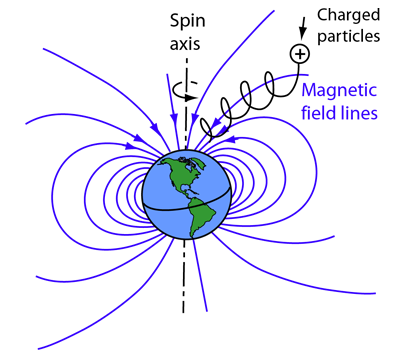
\includegraphics[width=0.5\linewidth]{Pictures/aurore_boreale_hyperphysics.png} \\
    L'interaction entre champ magnétique terrestre et particules solaires chargées produit les aurores boréales. Source: Université de Géorgie.
    \end{center}
\end{encart}


\subsection{Conservation du flux du champ magnétique}

Le champ magnétique présente également une propriété très importante :
\begin{theorem}[Conservation du flux]
    Le flux du champ magnétique à travers une surface fermée est nul.
\end{theorem}
C'est un postulat fondamental réalisé au XIXe siècle qui ne se démontre pas. Le postulat se justifie par le fait qu'il permet d'expliquer un grand nombre d'observations et de résultats d'expériences.

Cette propriété de conservation du flux est la même que celle pour un champ électrique dans une région vide de charges, sauf que pour le champ magnétique, elle est valable \textbf{partout} y compris dans les régions où des courants électriques sont présents. De la même manière que pour le champ électrique, en choisissant un tube de champ approprié, on peut alors montrer que :
\begin{proposition}
    Plus les lignes de champ magnétique sont resserrées, plus le champ magnétique est intense.
\end{proposition}

\section{Géométrie du champ magnétique créé par un courant}

Maintenant que nous avons bien défini courant électrique et champ magnétique, nous pouvons nous atteler à mieux décrire le lien entre les deux.

\subsection{La règle de la main droite}

Ce lien, comme nous l'avons vu, a été découvert par le danois {\O}rsted. En particulier, il a pu constater que le champ magnétique créé par un fil parcouru par un courant est :
\begin{itemize}
    \item Orthogonal au fil
    \item Dans le plan normal au fil
\end{itemize}
Autrement dit, le champ magnétique tourne autour du fil. L'expérience montre que le champ est orienté selon ce que l'on appelle la règle de la main droite (cf figure \ref{fig:main_droite}). Par exemple, dans un repère cylindrique de coordonnées $(r,\theta,z)$, si le courant parcourt l'axe $(Oz)$ dans le sens de $\vv{e_z}$, alors le champ magnétique est orienté dans le sens de $\vv{e_\theta}$. Par ailleurs, le français André-Marie Ampère a par la suite montré que l'amplitude du champ magnétique diminuait avec la distance au fil.

\begin{figure}[htbp]
    \centering
    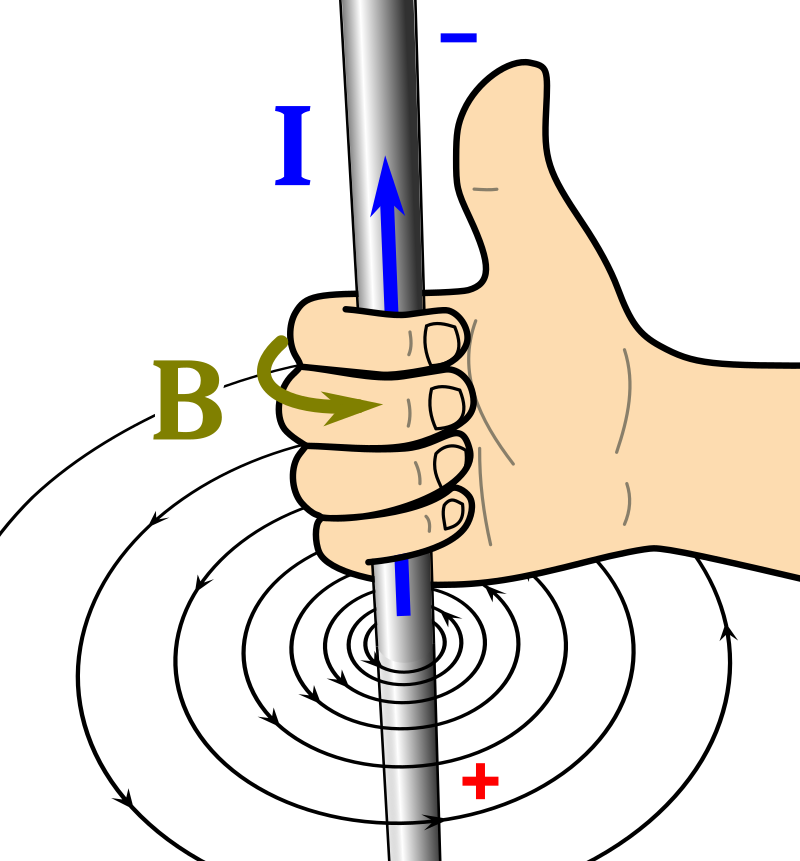
\includegraphics[width=0.3\linewidth]{Pictures/regle_de_la_main_droite.png}
    \caption{La règle de la main droite. Source : Wikimedia Commons.}
    \label{fig:main_droite}
\end{figure}

\begin{encart}[Détection de la foudre]
    La "règle de la main droite", autrement dit les propriétés d'orientation du champ magnétique mises en évidence par l'expérience d'{\O}rsted, sont utilisées pour la détection de la foudre. En effet, un éclair est parcouru par un courant de forte intensité. En supposant que l'éclair est vertical, celui-ci produit un champ magnétique orthoradial qui peut être mesuré par un réseau de stations en surface. En mesurant la direction du champ magnétique, on peut remonter à la direction de l'éclair. Avec plusieurs stations, on obtient plusieurs droites à l'intersection desquelles se trouve l'éclair.

    Ce type de réseau est très utilisé, d'une part pour la surveillance des événements météorologiques (notamment en Europe et aux États-Unis), et d'autre part pour des questions de recherche fondamentale. Dans les années 2010 par exemple, des équipes brésiliennes de chercheurs et chercheuses ont installé un réseau de détection dans l'Amazonie, l'une des régions où l'on enregistre le plus d'éclairs sur Terre.
\end{encart}

\begin{figure}[htbp]
    \centering

    \begin{tikzpicture}[scale=0.7]
    \coordinate (O) at (0,0);
    \coordinate (A) at (-3,3);
    \coordinate(B) at (1,2);

    \draw[dashed] (-1,-2) -- (2.5,5) node[anchor=west]{$\mathcal{D}_2$};
    \draw[dashed] (-4,4) -- (2,-2) node[anchor=west]{$\mathcal{D}_1$};

    \draw[-stealth,ultra thick] (A) --++ (1,1) node[anchor=west]{$\vv{B_1}$};
    \draw[-stealth,ultra thick] (B) --++ (2,-1) node[anchor=west]{$\vv{B_2}$};

    \draw (-2.8,3.2) -- (-3,3.4) -- (-3.2,3.2);
    \draw (1.3,1.85) -- (1.15,1.55) -- (0.85,1.7);

    \filldraw[yellow] (O) circle (0.3);
    \draw[] (O) circle (0.3) node[anchor=east]{\'eclair\,\,};
    \filldraw (B) circle (0.1) node[anchor=east]{$S_2$};
    \filldraw (A) circle (0.1) node[anchor=north]{$S_1$};
    \end{tikzpicture} 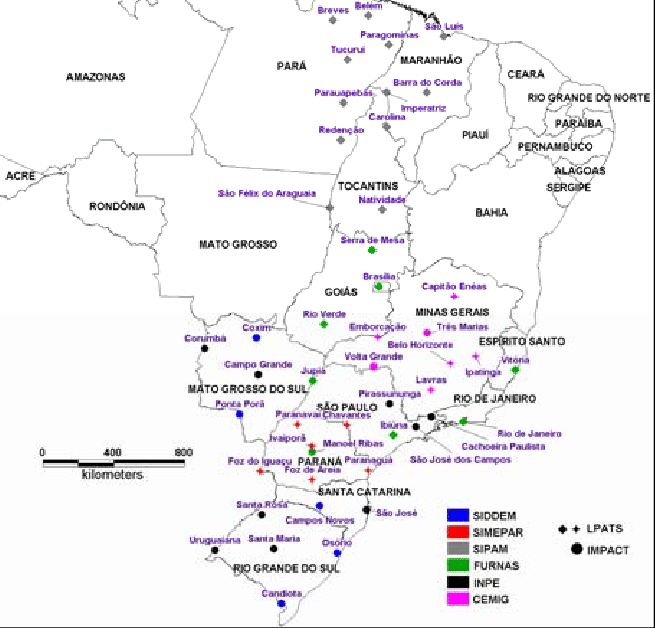
\includegraphics[width=0.4\linewidth]{Pictures/brasilDAT.png}
    \caption{A gauche : principe de détection des éclairs par la technique MDF (magnetic direction finding). Deux stations de mesure enregistrent des champs magnétiques $\vv B_1$ et $\vv B_2$. L'éclair se situe sur les droites $\mathcal{D}_1$ et $\mathcal{D}_2$ perpendiculaires aux champs mesurés. A droite : carte du réseau BrasilDAT de détection des éclairs au Brésil. Source : Naccataro et Pinto (2008).}
    \label{fig:lightning}
\end{figure}

Ces propriétés nous permettent, de manière plus générale, d'établir des liens entre les symétries d'une distribution de courant, et la symétrie du champ magnétique créé. Nous rappelons ici le principe de Curie :
\begin{theorem}[Principe de Curie]
    Les effets ont les symétries des causes
\end{theorem}

\paragraph{Invariances}

Les propriétés liées aux invariances découlent directement du principe de Curie et sont inchangées par rapport au champ électrostatique :
\begin{proposition}[Invariance par translation]
    Si la distribution de courants est invariante par translation selon un axe, alors le champ magnétique est indépendant de la coordonnée le long de cet axe.
\end{proposition}

\begin{proposition}[Invariance par rotation autour d'un axe]
    Si la distribution de courants est invariante par rotation autour d'un axe, alors dans le système de coordonnées polaires autour de cet axe, les composantes du champ magnétique ne dépendent pas de l'angle de rotation autour de cet axe.
\end{proposition}

Le cas de l'invariance par rotation autour d'un point n'est pas très adapté aux distributions de courants, puisque celles-ci sont généralement filiformes.

\paragraph{Symétries}

Dans le cas des symétries, la situation est différente de l'électrostatique, car le champ magnétique créé par un courant dépend de la direction de ce courant. Nous allons donc analyser à nouveau l'impact des symétries sur le champ.

\begin{figure}[htbp]
    \centering

    \begin{tikzpicture}[scale=0.3]

    \coordinate (A) at (-4,4);
    \coordinate (B) at (4,4);
    \coordinate (C) at (0,-4);
    \coordinate (D) at (-8,0);
    \coordinate (E) at (8,0);

    \draw[thick] (0,-8) -- (0,8) node[anchor=west]{$\Pi_s$};

    \draw[thick,dashed,blue] (D) -- (B);
    \draw[thick,dashed,blue] (E) -- (A);
    \draw[thick,dashed,yellow] (D) -- (A);
    \draw[thick,dashed,yellow] (E) -- (B);
    \draw[thick,dashed,green] (D) -- (C);
    \draw[thick,dashed,green] (E) -- (C);
    
    \draw[ultra thick,-stealth,blue] (A) --++(-.5,-2);
    \draw[ultra thick,-stealth,blue] (B) --++(-.5,2);
    \draw[ultra thick,-stealth,yellow] (B) --++(-3,-3);
    \draw[ultra thick,-stealth,yellow] (A) --++(-3,3);
    \draw[ultra thick,-stealth,green] (C) --++(1.5,3);
    \draw[ultra thick,-stealth,green] (C) --++(1.5,-3);
    \draw[ultra thick,-stealth,red] (C) --++(3,0) node[anchor=west]{$\vv B$};
    \draw[ultra thick,-stealth,red] (A) --++(-3.5,1) node[anchor=east]{$\vv B$};
    \draw[ultra thick,-stealth,red] (B) --++(-3.5,-1) node[anchor=south]{$\vv B$};
    \draw[dotted,red] (1.5,-1) -- (3,-4) -- (1.5,-7);
    \draw[dotted,red] (-4.5,2) -- (-7.5,5) -- (-7,7);
    \draw[dotted,red] (3.5,6) -- (0.5,3) -- (1,1);

    \filldraw (A) circle (0.15);
    \filldraw (B) circle (0.15);
    \filldraw (C) circle (0.15);
    \filldraw (D) circle (0.15);
    \draw[thick] (D) circle (0.5) node[anchor=east]{$i$\,};
    \filldraw (E) circle (0.15);
    \draw[thick] (E) circle (0.5) node[anchor=west]{\,$i$};
    \end{tikzpicture} \hspace{0.1\textwidth} \begin{tikzpicture}[scale=0.3]

    \coordinate (A) at (-4,4);
    \coordinate (B) at (4,4);
    \coordinate (C) at (0,-4);
    \coordinate (D) at (-8,0);
    \coordinate (E) at (8,0);

    \draw[thick] (0,-8) -- (0,8) node[anchor=west]{$\Pi_a$};

    \draw[thick,dashed,blue] (D) -- (B);
    \draw[thick,dashed,blue] (E) -- (A);
    \draw[thick,dashed,yellow] (D) -- (A);
    \draw[thick,dashed,yellow] (E) -- (B);
    \draw[thick,dashed,green] (D) -- (C);
    \draw[thick,dashed,green] (E) -- (C);
    
    \draw[ultra thick,-stealth,blue] (A) --++(.5,2);
    \draw[ultra thick,-stealth,blue] (B) --++(-.5,2);
    \draw[ultra thick,-stealth,yellow] (B) --++(3,3);
    \draw[ultra thick,-stealth,yellow] (A) --++(-3,3);
    \draw[ultra thick,-stealth,green] (C) --++(1.5,3);
    \draw[ultra thick,-stealth,green] (C) --++(-1.5,3);
    \draw[ultra thick,-stealth,red] (C) --++(0,6) node[anchor=west]{$\vv B$};
    \draw[ultra thick,-stealth,red] (A) --++(-2.5,5) node[anchor=east]{$\vv B$};
    \draw[ultra thick,-stealth,red] (B) --++(2.5,5) node[anchor=south]{$\vv B$};
    \draw[dotted,red] (1.5,-1) -- (0,2) -- (-1.5,-1);
    \draw[dotted,red] (-3.5,6) -- (-6.5,9) -- (-7,7);
    \draw[dotted,red] (3.5,6) -- (6.5,9) -- (7,7);

    \filldraw (A) circle (0.15);
    \filldraw (B) circle (0.15);
    \filldraw (C) circle (0.15);
    \filldraw (D) circle (0.15);
    \draw[thick] (D) circle (0.5) node[anchor=east]{$i$\,};
    \draw (8-.353,-.353) -- (8+.353,.353);
    \draw (8-.353,.353) -- (8+.353,-.353);
    \draw[thick] (E) circle (0.5) node[anchor=west]{\,$i$};
    \end{tikzpicture}
    
    \caption{Plans de symétrie et d'antisymétrie de la distribution de courants. Les fils sont parcourus par un même courant $i$ et orientés perpendiculairement au plan du schéma et la direction du courant (vers l'avant ou vers l'arrière) est indiquée par le symbole associé. Les distances identiques sont indiquées avec des tirets de même couleur. Le champ magnétique produit par chaque point est dessiné en suivant la règle de la main droite. Les composantes du champ magnétique de même norme sont également indiquées de la même couleur. Le champ magnétique total est indiqué en rouge.}
    \label{fig:plans_symetrie}
\end{figure}

\begin{proposition}[Plan de symétrie de la distribution de courants]
    Un plan de symétrie de la distribution de courants est un plan d'antisymétrie du champ magnétique. En particulier, le vecteur champ magnétique en tout point de ce plan est normal à ce plan.
\end{proposition}

\begin{proposition}[Plan d'antisymétrie de la distribution de courants]
    Un plan d'antisymétrie de la distribution de courants est un plan de symétrie du champ magnétique. En particulier, le vecteur champ magnétique en tout point de ce plan est contenu dans ce plan.
\end{proposition}

De la même manière qu'en électrostatique, ces propriétés pourront être utilisées pour déterminer la forme du champ magnétique. 

\section{Théorème d'Ampère}

Pour l'instant, nous avons, à partir des résultats de l'expérience d'{\O}rsted, établi des règles qui nous permettent de déterminer l'orientation du champ magnétique créé par une distribution de courants en tout point de l'espace. C'est ensuite André-Marie Ampère qui a mené des expérience méthodiques pour étudier de manière quantitative le champ magnétique créé par un courant. Ses travaux ont permis, plus tard, de démontrer ce que l'on appelle aujourd'hui le théorème d'Ampère. Il s'agit d'une loi empirique entièrement basée sur des résultats expérimentaux :
\begin{theorem}[Théorème d'Ampère]
    Soit un contour fermé et orienté $\Gamma$. La circulation du champ magnétique le long de ce contour est reliée au courant $I_{\mathrm{enlace}}$ enlacé par le contour selon la loi suivante :
    \begin{equation}
        \oint \vv B \cdot \vv{\dd \ell} = \mu_0 I_{\mathrm{enlace}}
    \end{equation}
    où $\mu_0 = 4 \pi \times 10^{-7}\,$T$\cdot$m$\cdot$A$^{-1}$ est la perméabilité magnétique du vide.
\end{theorem}

Le courant enlacé par le contour est définit comme l'intensité qui traverse une surface $\Sigma$ s'appuyant sur le contour, et orientée par convention selon la règle de la main droite :
\begin{equation}
    I_{\mathrm{enlace}} = \iint_\Sigma \vv j \cdot \vv{\dd S}
\end{equation}

Le théorème d'Ampère, comme le théorème de Gauss, ne nous donne pas directement le champ magnétique, mais une grandeur intégrale et macroscopique reliée à ce champ. Alors que le théorème de Gauss fournit le flux du champ électrique à travers une surface fermée, le théorème d'Ampère fournit la circulation du champ magnétique le long d'un contour fermé. Cette différence géométrique est appropriée à la géométrie différente des distributions qui créent les champs : le champ électrique est créé par des charges de géométrie ponctuelle, alors que le champ magnétique est créé par des courants souvent répartis le long de fils ayant une structure linéaire.

Comme pour le théorème de Gauss, c'est en combinant l'analyse des symétries d'un problème et le théorème d'Ampère que l'on pourra établir une expression pour le champ magnétique. En particulier, lorsque la symétrie de la distribution de courants n'est pas suffisante, il est possible de décomposer cette distribution en distributions plus simples et d'appliquer le principe de superposition :

\begin{proposition}[Principe de superposition]
Soient deux distributions de courants $\mathcal{D}_1$ et $\mathcal{D}_2$, créant des champs magnétiques respectifs $\vv B_1$ et $\vv B_2$. Le champ magnétique créé par la distribution $\mathcal{D}_1 \cup \mathcal{D}_2$ est alors $\vv B = \vv B_1 + \vv B_2$.
\end{proposition}

Dans la suite, nous allons voir quelques applications classiques du théorème d'Ampère.

\subsection{Application : fil électrique infini}

\begin{figure}
    \centering


\tdplotsetmaincoords{70}{100}
\begin{tikzpicture}[scale=3,tdplot_main_coords]
  
  % VARIABLE
  \def\t{0.01}
  \def\Rin{0.7}
  \def\Rout{0.74}
  \def\Bpara{0.26}
  \def\Bperp{0.24}
  \def\rvec{1.3}
  \def\thetavec{90}
  \def\phivec{40}
  \def\dtheta{10}
  \def\dphi{15}
  \def\R{0.85}
  \def\B{0.5}
  \def\zp{1}
  \def\Rp{1.35}
  \coordinate (O) at (0,0,0);
  \coordinate (P) at ({\Rin*cos(\phivec)},{\Rin*sin(\phivec)},{1.4*\t*cos(\phivec)});
  \coordinate (P0) at (0:0.96*\Rin);
  \coordinate (X) at (0,0,1.0*\Rin);
  \coordinate (BY) at ({\Bpara*cos(\phivec)},{\Bpara*sin(\phivec)},1.0*\Rin);
  \coordinate (BX) at (0,0,1.0*\Rin+\Bperp);
  \coordinate (B) at ({\Bpara*cos(\phivec)},{\Bpara*sin(\phivec)},1.0*\Rin+\Bperp);
  \coordinate (M) at ({\R*cos(\phivec)*sin(\thetavec)},{\R*sin(\phivec)*sin(\thetavec)},{\R*cos(\thetavec)});
   \coordinate (MB) at ({\R*cos(\phivec)*sin(\thetavec)-\B*sin(\phivec)},{\R*sin(\phivec)*sin(\thetavec)+\B*cos(\phivec)},{\R*cos(\thetavec)});
  \coordinate (M1) at ({\Rp*cos(\phivec)},{\Rp*sin(\phivec)},-\zp);
  \coordinate (M2) at ({\Rp*cos(\phivec)},{\Rp*sin(\phivec)},\zp);
  \coordinate (M3) at ({-\Rp*cos(\phivec)},{-\Rp*sin(\phivec)},\zp);
  \coordinate (M4) at ({-\Rp*cos(\phivec)},{-\Rp*sin(\phivec)},-\zp);

  
  \draw[black] (0,0,-1.5*\Rin) -- (0,0,0) ;
\draw[black!50,ultra thick,->] (0,0,-\Rin) -- (0,0,-0.1) node[anchor=east]{$i$} ;


  %WIRE
  \draw[ultra thick,black] (O) circle (1.15*\Rout);

  \tdplotsetthetaplanecoords{\phivec}
  \draw[tdplot_rotated_coords,myred]  (M1) -- (M2) -- (M3) -- (M4) -- (M1) node[anchor=west]{$\Pi_s$};
  \draw[->] (0,0,0) -- (0,0,1.55*\Rin) node[anchor=west]{$z$};
\draw[black!50,ultra thick] (0,0,-0.2) -- (0,0,1.3*\Rin);
  \draw[->,thick] (O) -- (M) node[midway,anchor=south]{$r$};
  \draw[->,ultra thick,myred] (M) -- (MB) node[anchor=west]{$\vv B$};
  \draw[current,domain=0:40,samples=10, ultra thick]
    (-40:1.15*\Rout) arc (-40:-10:1.15*\Rout) node[below] {$\Gamma$};
  \filldraw[tdplot_rotated_coords] (M) circle (0.02) node[anchor=north]{$M$};
\end{tikzpicture} 

    \caption{Fil infini parcouru par un courant $i$ (en gris au centre). Le contour d'Ampère choisi est le cercle noir. Un plan de symétrie de la distribution de courants est également indiqué.}
    \label{fig:fil_infini}
\end{figure}


Considérons un fil infini parcouru par un courant constant $i$. Nous nous plaçons dans le repère de coordonnées cylindriques $(r,\theta,z)$ dont l'axe $(Oz)$ coïncide avec le fil, et tel que le courant circule dans le sens $+\vv{e_z}$.

Nous commençons par utiliser le principe de Curie. La distribution de courants est invariante par translation selon $\vv{e_z}$ et par rotation autour de $(Oz)$, ainsi les composantes du champ magnétique ne dépendent pas de $z$ ni de $\theta$.

Par ailleurs, considérons un point $M$ quelconque. Le plan contenant $M$ et $(Oz)$ est un plan de symétrie de la distribution de courants. C'est donc un plan d'antisymétrie du champ magnétique. En particulier, le champ magnétique au point $M$ est normal à ce plan. Ce plan contient les vecteurs $\vv{e_r}$ et $\vv{e_z}$, et $\vv{B}(M)$ est normal à ce plan, donc $\vv{B}(M)$ est orienté selon $\vv{e_\theta}$.

On conclut que le champ magnétique est de la forme :
\begin{equation}
    \vv B = B(r) \vv{e_\theta}
\end{equation}

\begin{remark}
    On peut aussi remarquer que le plan passant par $M$ et perpendiculaire à $(Oz)$ est un plan d'antisymétrie de la distribution de courants, et donc un plan de symétrie du champ magnétique. Le champ magnétique est donc contenu dans ce plan, c'est-à-dire que sa composante selon $\vv{e_z}$ est nulle.

    Mais comme on le voit plus haut, ce n'était pas nécessaire pour conclure, et trouver un plan de symétrie permet d'avoir un résultat plus précis (on obtient en un seul coup l'orientation du champ).
\end{remark}

\begin{capex}
En appliquant le théorème d'Ampère au contour $\Gamma$ indiqué sur la figure \ref{fig:fil_infini}, déterminer l'expression du champ magnétique autour du fil.
\end{capex}

%Nous choisissons maintenant un contour fermé approprié à la situation : soit $\Gamma$ le cercle passant par $M$, de rayon $r$ et orienté selon $+\vv{e_\theta}$. Le courant enlacé par ce contour est tout simplement le courant $i$ parcouru par le fil. Par ailleurs, la circulation du champ magnétique le long de ce contour est donnée par :
%\begin{equation}
%    \oint_\Gamma \vv B \cdot \vv{\dd \ell} = \int_0^{2\pi} B(r) \times r \dd \theta = 2 \pi r B(r)
%\end{equation}
%Le théorème d'Ampère s'écrit :
%\begin{equation}
%    \oint_\Gamma \vv B \cdot \vv{\dd \ell} = \mu_0 I_{\mathrm{enlace}}
%\end{equation}
%et on obtient donc :
%\begin{equation}
%    2 \pi r B(r) = \mu_0 i
%\end{equation}
%ou encore :
%\begin{equation}
%    \vv B = \frac{\mu_0 i}{2 \pi r} \vv{e_\theta}
%\end{equation}

\begin{remark}
    Cet exemple est très classique. Il est vivement recommandé de connaître le résultat par coeur et de savoir le retrouver facilement.
\end{remark}

\subsection{Application : solénoïde infini}

\begin{figure}[htbp]
    \centering

\begin{tikzpicture}[scale=1.3]
  \def\R{1}
  \def\N{12}
  \def\NB{4}
  \def\L{6}
  \def\t{0.20*\R}
  \def\w{\L/(\N-1)}
  %\draw[current] (-0.6*\R,-0.01*\R) arc (-94:-86:{0.6*\R/sin(4)})
  %  node[midway,below=0.6] {\contour{white}{$I$}};

  \draw[->] (.75*\L,1.4*\R) --++(0.65,0) node[anchor=north]{$\vv{e_z}$};
  \draw[->] (.75*\L,1.4*\R) --++(0.,0.65) node[anchor=east]{$\vv{e_r}$};
  \pic[scale=0.81] at (.75*\L,1.4*\R) {Bout={Icol}};
  \node[anchor=east] at (.75*\L,1.4*\R) {$\vv{e_\theta}$} ;

  
  \draw[->] (.75*\L,-1.4*\R) --++(0.65,0) node[anchor=north]{$\vv{e_z}$};
  \draw[->] (.75*\L,-1.4*\R) --++(0.,-0.65) node[anchor=east]{$\vv{e_r}$};
  \pic[scale=0.81] at (.75*\L,-1.4*\R) {Bin={Icol}};
  \node[anchor=east] at (.75*\L,-1.4*\R) {$\vv{e_\theta}$} ;

  \draw[<->] (-0.5*\L,-1.3*\R) -- (0.6*\L,-1.3*\R) node[midway,anchor=north]{$\ell$};
  \draw[<->] (-0.27*\L,2*\R) -- (0.27*\L,2*\R) node[midway,anchor=south]{$L$};
  
  % WIRE BACK
  \foreach \i [evaluate={\x=-\L/2+(\i-1)*\w; \ang=atan(4*\R/(\w));}] in {1,...,\N}{
    \ifthenelse{\i<\N}{
      \draw[lightmetal]
        ({\x+\w/2},-\R)++(\ang+90:\t/2) to[out=\ang+5,in=\ang-185]++ (\ang:2.02*\R) -- ({\x+\w},\R) --++ (\ang-90:\t/2) to[out=\ang-185,in=\ang+5]++ (\ang-180:2.02*\R) -- cycle;
    }{}
  }
  
  % MAGNETIC FIELDLINES
  \foreach \i [evaluate={\y=(\i-\NB/2-0.5)*1.4*\R/\NB}] in {1,...,\NB}{
      \draw[BFieldLine={0.505}] (-0.55*\L,\y) -- (0.62*\L,\y);
  }
  \node[Bcol] at (0.61*\L,0.76*\R) {$\vv{B}$};

  \draw[->,thick] ({-0.8*\L},0) -- ({0.85*\L},0) node[anchor=north]{$z$};

\draw[dotted] (-0.7*\L,0.6*\R) -- (-0.27*\L,0.6*\R);
\draw[dotted] (-0.8*\L,1.8*\R) -- (-0.27*\L,1.8*\R);
\draw[dotted] (-0.7*\L,-\R) -- (-\L/2.15,-\R);
\draw[<->] (-0.6*\L,0) -- (-0.6*\L,0.6*\R) node[midway,anchor=east]{$r_1$};
\draw[<->] (-0.75*\L,0) -- (-0.75*\L,1.8*\R) node[midway,anchor=east]{$r_2$};
\draw[<->] (-0.675*\L,0) -- (-0.675*\L,-\R) node[midway,anchor=east]{$R$};

  
  % AMPERE's LOOP
  \draw[Ampcol]
    (-0.27*\L,0.6*\R) -| (0.27*\L,1.8*\R) -| cycle;
  \draw[Ampcurve={0.54}]
    (-0.27*\L,0.6*\R) -- (0.27*\L,0.6*\R) ;
  \draw[Ampcurve={0.68}]
    ( 0.27*\L,0.6*\R) -- (0.27*\L,1.8*\R) node[anchor=west]{$\Gamma$} ;
  \draw[Ampcurve={0.55}]
    ( 0.27*\L,1.8*\R) -- (-0.27*\L,1.8*\R);
  \draw[Ampcurve={0.57}]
    (-0.27*\L,1.8*\R) -- (-0.27*\L,0.6*\R) ;
  
  % WIRE FRONT
  \foreach \i [evaluate={\x=-\L/2+(\i-1)*\w; \ang=atan(4*\R/(\w));}] in {1,...,\N}{
    \draw[metal] (\x,\R)++(-90-\ang:\t/2) --++ (90-\ang:\t) to[out=-\ang-5,in=185-\ang]++ (-\ang:2.02*\R) -- ({\x+\w/2},-\R) --++ (-90-\ang:\t/2) to[out=185-\ang,in=-\ang-5] cycle;
    \pic[scale=1.05] at ({\x+\w/2},-\R) {Bin={Icol}};
    \pic[scale=1.05] at (\x,\R) {Bout={Icol}};
  }
  \node[Icol] at (-0.545*\L,1.02*\R) {$i$};

    
\end{tikzpicture}

    
    \caption{Le solénoïde infini}
    \label{fig:placeholder}
\end{figure}

Considérons maintenant un exemple qui a de nombreuses applications pratiques : une bobine de fil parcourue par un courant. Ce type de bobine est présent notamment dans les moteurs et dans de très nombreux circuits électriques. Vous avez déjà vu le comportement électrique d'une bobine en MPSI, et nous allons essayer de le démontrer ici à partir du théorème d'Ampère. Nous allons, pour simplifier le problème, supposer que nous nous trouvons loin des bords de la bobine, ce qui nous permet de supposer qu'elle est infinie dans le sens de la longueur. On parle du solénoïde infini. Nous notons $i$ le courant circulant dans la bobine, et $R$ le rayon des spires\footnote{Une spire est une boucle de courant.}. On suppose que les spires sont jointives (elles se touchent) et on note $n$ le nombre de spires par unité de longueur.

Nous adoptons à nouveau un système de coordonnées cylindriques dont l'axe coïncide avec l'axe de la bobine. L'axe $(Oz)$ est orienté de telle sorte que le courant circule selon la direction $+\vv{e_\theta}$.

\begin{capex}
Par une analyse des symétries du problème, déterminer la forme du champ magnétique.
\end{capex}

%Commençons par analyser les symétries du problème. Le problème est invariant par rotation autour de $(Oz)$ et par translation selon $\vv{e_z}$, ainsi les composantes du champ magnétique ne dépendent que du rayon $r$.
%
%Par ailleurs, soit $M$ un point quelconque de l'espace. Le plan passant par $M$ et perpendiculaire à l'axe $(Oz)$ est un plan de symétrie de la distribution de courants. Il s'agit donc d'un plan d'antisymétrie du champ magnétique. Le champ $\vv B(M)$ est donc normal à ce plan.
%
%On en conclut que le champ magnétique est de la forme :
%\begin{equation}
%    \vv B = B(r) \vv{e_z}
%\end{equation}

Nous allons maintenant choisir un contour approprié. Nous prenons un contour rectangulaire dans le plan $\theta=0$, de longueur $L$ selon l'axe $(Oz)$, et situé entre les rayons $r_1$ et $r_2$. Nous supposons que $r_2 \gg R$ si bien que l'on se trouve très loin de la bobine. On peut alors supposer que $B(r_2) = 0$. Nous choisissons le contour orienté dans le sens trigonométrique, selon $+\vv{e_z}$ en $r=r_1$. 

\begin{capex}
En appliquant le théorème d'Ampère à ce contour, déterminer le champ magnétique à l'intérieur et à l'extérieur de la bobine.
\end{capex}

%La circulation du champ magnétique le long de ce contour est donnée par :
%\begin{equation}
%    \oint_\Gamma \vv B \cdot \vv{\dd \ell} = B(r_1) L - B(r_2) L = B(r_1) L
%\end{equation}
%car on a choisi $r_2 \gg R$ de sorte que $B(r_2) = 0$.
%Par ailleurs, le courant enlacé par le contour correspond au courant $i$ de la bobine multiplié par le nombre de spires enlacées $N = n \times L$. Les spires ne sont enlacées par le contour que si $r_1<R$. Ainsi :
%\begin{itemize}
%    \item Si $r_1<R$ alors $I_{\mathrm{enlace}} = i n L$
%    \item Sinon $I_{\mathrm{enlace}} = 0$
%\end{itemize}
%Nous appliquons le théorème d'Ampère :
%\begin{equation}
%    \oint_\Gamma \vv B \cdot \vv{\dd \ell} = \mu_0 I_{\mathrm{enlace}}
%\end{equation}
%et nous obtenons le champ à l'intérieur de la bobine :
%\begin{equation}
%    \vv B = \mu_0 n i \vv{e_z} \quad \mathrm{si} \quad r<R
%\end{equation}
%alors que le champ est nul à l'extérieur de la bobine.

\begin{remark}
    Ce résultat est à connaître. Il faut savoir le démontrer. Attention à l'orientation des contours et des vecteurs, bien utiliser la règle de la main droite.
\end{remark}

\begin{capex}
Après avoir rappelé la définition de l'inductiance $L$, calculer l'inductance de la bobine en fonction de $R,N$ et $\ell$.
\end{capex}

%Nous avons vu en première année la relation $\Phi = L i$ entre le flux du champ magnétique à travers les spires d'une bobine et le courant qui la parcourt. Nous pouvons maintenant calculer l'inductance d'une bobine en fonction de ses propriétés.
%
%Comme le champ magnétique est uniforme à l'intérieur du solénoïde, le flux du champ magnétique à travers une spire de la bobine est directement donné par une multiplication (pas besoin de calculer une intégrale) :
%\begin{equation}
%    \Phi_{\mathrm{1\,spire}} = \pi R^2 \times B = \mu_0 n i \pi R^2
%\end{equation}
%Supponsons maintenant que la bobine contient $N$ spires. Le flux total à travers la bobine est donné par $\Phi = N \Phi_{\mathrm{1\,spire}}$. En remarquant que $n = N/\ell$ où $\ell$ est la longueur de la bobine, nous obtenons l'expression de son inductance :
%\begin{equation}
%    \Phi = L i \quad \mathrm{avec} \quad L = \frac{\pi \mu_0 R^2 N^2}{\ell}
%\end{equation}

Nous allons maintenant supposer que le courant électrique dans la bobine varie avec le temps, ainsi le champ magnétique produit par ce courant va également varier. Dans ce cas, nous ne sommes plus stricto sensu en régime permanent et les lois de la magnétostatique ne sont a priori plus valides. Mais, nous pouvons nous placer dans le cadre de l'ARQS magnétique, c'est-à-dire que nous supposons que le courant varie lentement par rapport au temps caractéristique avec lequel le champ magnétique est influencé par le courant. Ainsi, on peut considérer que le champ magnétique peut être approximé par les lois de la magnétostatique. Nous verrons plus en détail les conditions exactes d'application de l'ARQS plus tard dans l'année.

Revenons maintenant à la bobine, qui est traversée par un champ $B$ qui varie avec le temps. Par les lois de l'induction, une force électromotrice apparaît aux bornes de la bobine lorsque le flux du champ magnétique varie. On rappelle la loi de l'induction vue en première année :

\begin{theorem}[Loi de Faraday (Rappel de MPSI)]
    Soit une portion de circuit orientée, traversée par un champ magnétique variable. Nous notons $\Phi$ le flux du champ magnétique à travers cette portion de circuit. Ceci conduit à l'apparition d'une force électromotrice, dans le sens d'orientation du circuit :
    \begin{equation}
        e = - \frac{\dd \Phi}{\dd t}
    \end{equation}
\end{theorem}

Nous pouvons appliquer la loi de Faraday à la bobine. Nous avons choisi d'orienter le solénoïde dans le sens du courant. En convention récepteur, la tension est orientée dans le sens opposé au courant, et elle est donc donnée par :
\begin{equation}
    u = -e = \frac{\dd \Phi}{\dd t}
\end{equation}
On en déduit que la tension aux bornes du solénoïde est donnée par :
\begin{equation}
    u = L \frac{\dd i}{\dd t}
\end{equation}
Nous avons ainsi démontré la loi courant-tension des bobines à partir des lois de la magnétostatique et de l'induction. L'inductance $L$ augmente avec le carré du nombre de spires, ainsi en augmentant ce nombre de spires on peut rapidement atteindre des inductances très élevées.

\begin{remark}
    Dans tous ces calculs, nous avons supposé le solénoïde infini, nous négligeons donc les effets de bord. En réalité, le rayon et la longueur d'une bobine sont souvent comparables, si bien que les calculs réalisés ici ne donnent qu'un ordre de grandeur des propriétés de la bobine.
\end{remark}

\begin{remark}
    L'analyse du solénoïde infini a été l'opportunité de faire quelques rappels de MPSI sur l'induction. En particulier nous avons revu le cas d'un circuit fixe placé dans un champ magnétique dépendant du temps. Le cas contraire (un circuit mobile dans un champ magnétique constant) a été abordé en première année, nous ferons quelques révisions en TD à travers l'exemple des rails de Laplace.
\end{remark}


\section{Le dipôle magnétique}

Maintenant que nous avons établi un lien entre courant électrique et champ magnétique, et étudié quelques situations classiques, nous pouvons nous intéresser au champ produit par une unique boucle de courant de rayon $a$.

\begin{figure}[htbp]
    \centering


\tdplotsetmaincoords{70}{100}
\begin{tikzpicture}[scale=3,tdplot_main_coords]
  
  % VARIABLE
  \def\t{0.01}
  \def\Rin{0.7}
  \def\Rout{0.74}
  \def\Bpara{0.26}
  \def\Bperp{0.24}
  \def\rvec{1.3}
  \def\thetavec{50}
  \def\phivec{70}
  \def\dtheta{10}
  \def\dphi{15}
  \def\R{1.3}
  \def\zp{1}
  \def\Rp{1.35}
  \coordinate (O) at (0,0,0);
  \coordinate (P) at ({\Rin*cos(\phivec)},{\Rin*sin(\phivec)},{1.4*\t*cos(\phivec)});
  \coordinate (P0) at (0:0.96*\Rin);
  \coordinate (X) at (0,0,1.0*\Rin);
  \coordinate (BY) at ({\Bpara*cos(\phivec)},{\Bpara*sin(\phivec)},1.0*\Rin);
  \coordinate (BX) at (0,0,1.0*\Rin+\Bperp);
  \coordinate (B) at ({\Bpara*cos(\phivec)},{\Bpara*sin(\phivec)},1.0*\Rin+\Bperp);
  \coordinate (M) at ({\R*cos(\phivec)*sin(\thetavec)},{\R*sin(\phivec)*sin(\thetavec)},{\R*cos(\thetavec)});
  \coordinate (M1) at ({\Rp*cos(\phivec)},{\Rp*sin(\phivec)},-\zp);
  \coordinate (M2) at ({\Rp*cos(\phivec)},{\Rp*sin(\phivec)},\zp);
  \coordinate (M3) at ({-\Rp*cos(\phivec)},{-\Rp*sin(\phivec)},\zp);
  \coordinate (M4) at ({-\Rp*cos(\phivec)},{-\Rp*sin(\phivec)},-\zp);

  
  \draw (0,0,-\Rin) -- (0,0,0) ;

  %WIRE
  \draw[shading=ring, ring color=black!60,domain=0:360,samples=120,even odd rule]
    plot ({\Rin*cos(\x)},{\Rin*sin(\x)},{\t*cos(\x)})
    plot ({\Rout*cos(\x)},{\Rout*sin(\x)},{-\t*cos(\x)});

  \tdplotsetthetaplanecoords{\phivec}
  \draw[tdplot_rotated_coords,myred]  (M1) -- (M2) -- (M3) -- (M4) -- (M1) node[anchor=west]{$\Pi_a$};
  \draw[->] (0,0,0) -- (0,0,1.55*\Rin) node[anchor=west]{$z$};
  \draw[->,thick] (O) -- (M) node[midway,anchor=east]{$r$};
  \draw[current,domain=0:40,samples=10]
    (-40:1.15*\Rout) arc (-40:-10:1.15*\Rout) node[midway,below] {$i$};
  \tdplotdrawarc[->,tdplot_rotated_coords]{(O)}{0.2*\Rin}{0}{atan(1.1)}{right=2,above=-1,scale=1}{\contour{white}{$\theta$}}
  \filldraw[tdplot_rotated_coords] (M) circle (0.02) node[anchor=west]{$M$};
\end{tikzpicture} 

    \caption{Etude des symétries dans le cas d'une spire parcourue par un courant $i$.}
    \label{fig:placeholder}
\end{figure}

Nous supposons la boucle placée à l'origine d'un repère sphérique $(r,\theta,\varphi)$. 

\begin{remark}
Il pourrait être tentant ici de choisir un système de coordonnées cylindriques, mais la pratique montre que les calculs sont en général plus simples en coordonnées sphériques (comme pour le dipôle électrostatique).
\end{remark}

\begin{capex}
Etablir la forme générale du champ magnétique par une analyse des symétries du problème.
\end{capex}

%Le problème étant invariant par rotation autour de $(Oz)$, les coordonnées du champ magnétique dans ce repère ne dépendent pas de $\varphi$. 
%
%Par ailleurs, considérons un point $M$ quelconque. Le plan $\Pi_a$ contenant $M$ et $(Oz)$ est un plan d'antisymétrie de la distribution de courants; c'est donc un plan de symétrie de la distribution de charges et on en déduit que $\vv B(M)$ est contenu dans ce plan. Ainsi :
%\begin{equation}
%    \vv B = B_r(r,\theta) \vv{e_r} + B_\theta(r,\theta) \vv{e_\theta}
%\end{equation}

Le degré de symétrie de la situation n'est pas suffisant pour obtenir une expression du champ magnétique simple. Nous ne pouvons donc pas calculer le champ magnétique créé par cette boucle de courant par le théorème d'Ampère. Pour simplifier les calculs, on se place à une distance grande par rapport à taille de la spire, c'est ce qu'on appelle l'approximation dipolaire magnétique :
\begin{definition}[Approximation dipolaire]
On parle d'approximation dipolaire lorsque l'on se place à une distance $r$ grande devant le rayon $a$ de la boucle de courant considérée : $r \gg a$.
\end{definition}
Dans le cadre de cette approximation, des calculs hors programme permettent de montrer que :
\begin{equation}
 \vv B = \frac{\mu_0 i S}{4 \pi r^3} ( 2 \cos \theta \vv{e_r} + \sin \theta \vv{e_\theta} )
\end{equation}
où $S = \pi a^2$ est la surface délimitée par la boucle de courant. 

\begin{figure}[htbp]
    \centering
    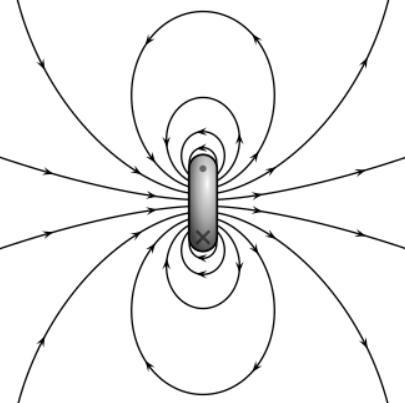
\includegraphics[height=0.4\linewidth]{Pictures/dipole_pres.png} 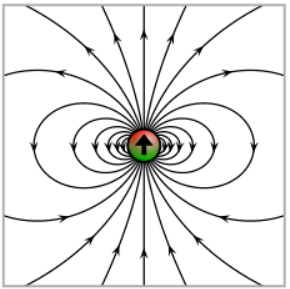
\includegraphics[angle=90,height=0.4\linewidth]{Pictures/dipole_loin.png}
    \caption{Le champ magnétique créé par une boucle de courant proche de la boucle (à gauche) et loin de la boucle, dans le cadre de l'approximation dipolaire (à droite). Source : Wikimedia Commons.}
    \label{fig:champ_dipolaire}
\end{figure}

On constate que cette expression est formellement analogue à l'expression du champ électrique créé par un dipôle électrostatique. On dira donc que la boucle de courant est un dipôle magnétique. On définit ainsi le moment magnétique d'une boucle de courant :
\begin{proposition}[Moment magnétique d'une spire (Rappel de MPSI)]
    Le moment magnétique d'une spire parcourue par un courant est donné par :
    \begin{equation}
    \vv{\mathcal{M}} = i S \vv n
    \end{equation}
    où $S$ est la surface de la spire, $\vv n$ le vecteur normal à la surface et $i$ le courant le long de la spire, orienté selon la règle de la main droite. Il se mesure en A$\cdot$m$^2$.
\end{proposition}

Ces lignes de champ sont également analogues à celles produites par un matériau aimanté. On peut ainsi définir un moment magnétique pour les aimants permanents, qui mesure l'intensité de cette circulation.

\subsection{Forces agissant sur un dipôle magnétique}

Nous pouvons maintenant nous interroger sur les forces agissant sur un dipôle magnétique. Pour cela, nous pouvons rappeler que dans circuit électrique, la force de Lorentz s'applique aux électrons en mouvement ce qui se traduit par une force de Laplace qui s'applique au circuit électrique :
\begin{proposition}[Force de Laplace (rappel de MPSI)]
    Soit un élément $\vv{\dd \ell}$ de circuit électrique parcouru par un courant $i$ et placé dans un champ magnétique $\vv B$. La résultante des forces magnétiques de Lorentz qui s'appliquent aux électrons du circuit se traduit par la force élémentaire de Laplace :
    \begin{equation}
        \vv{\dd F} = i \vv{\dd \ell} \wedge \vv B
    \end{equation}
\end{proposition}

Si nous appliquons cette loi à la boucle de courant placée dans un champ magnétique uniforme, nous pouvons constater qu'un couple s'exerce sur elle :
\begin{proposition}
    Une spire ou un aimant de moment magnétique $\vv{\mathcal{M}}$ placé dans un champ magnétique $\vv B$ subit un couple :
    \begin{equation}
        \vv \Gamma = \vv{\mathcal{M}} \wedge \vv B
    \end{equation}
\end{proposition}
\begin{demonstration}
\textit{Cette démonstration n'est pas explicitement au programme donc pas à connaître, mais elle est tout à fait faisable avec les outils que nous avons en MP.}
Pour le prouver, nous nous plaçons dans le repère de coordonnées sphériques d'origine $O$ le centre de la spire. Nous choisissons d'orienter la direction $\varphi=0$ selon la direction de la projection du champ $\vv B$ ambiant sur le plan $(xOy)$. En notant $\Theta$ l'angle entre $\vv B$ et $\vv{e_z}$ nous avons alors :
\begin{equation}
\vv B = B (\cos \Theta \vv{e_z} + \sin \Theta \vv{e_x})
\end{equation}
Par ailleurs, nous pouvons considérer un élément de longueur $\vv{d\ell}$ situé le long de la spire et repéré par sa coordonnée $\varphi$. On a $\vv{\dd \ell} = R \dd \varphi \vv{e_\varphi}$. La force de Laplace qui s'exerce sur cet élément est donnée par :
\begin{equation}
\dd \vv F = i \vv{\dd \ell} \wedge \vv B = i R \dd \varphi \vv{e_\varphi} \wedge \vv B 
\end{equation}
et le moment de cette force par rapport à $O$ s'écrit ainsi :
\begin{align}
\dd \vv \Gamma &= R \vv{e_r} \wedge \dd \vv F \\
&= i R^2 \dd \varphi \vv{e_r} \wedge (\vv{e_\varphi} \wedge \vv B) \\
&= i R^2 \dd \varphi ( (\vv{e_r} \cdot \vv B) \vv{e_\varphi} - (\vv{e_r} \cdot \vv{e_\varphi}) \vv B) \\
&= i R^2 \dd \varphi (\vv{e_r} \cdot \vv B) \vv{e_\varphi} \quad \mathrm{car} \quad \vv{e_r} \cdot \vv{e_\varphi} = 0 \\
&= i R^2 \dd \varphi B \sin \Theta \cos \varphi \vv{e_\varphi} \\
&= i R^2 \dd \varphi B \sin \Theta \cos \varphi (\cos \varphi \vv{e_y}-\sin \varphi \vv{e_x} + )
\end{align}
Le couple total exercé par les forces de Laplace vaut donc :
\begin{align}
\dd \vv \Gamma &= \int_0^{2\pi} \dd \vv \Gamma \\
&= i R^2  B \sin \Theta \int_0^{2\pi} \cos \varphi (\cos \varphi \vv{e_y} - \sin \varphi \vv{e_x}) \dd \varphi \\
&= i R^2  B \sin \Theta \left[ \left( \int_0^{2\pi} \cos^2 \varphi \dd \varphi \right) \vv{e_y} - \left( \int_0^{2\pi} \cos \varphi \sin \varphi \dd \varphi \right) \vv{e_x} \right] \\
&= i R^2  B \sin \Theta \times \pi \vv{e_y} \\
&= (i \pi R^2 \vv{e_z}) \wedge \vv B \\
&= \vv{\mathcal{M}} \wedge \vv B
\end{align}
\end{demonstration}

\begin{figure}[htbp]
    \centering

\begin{tikzpicture}[scale=1.3]
 
  % axes
  \coordinate (O) at (0,0);
  \coordinate (B) at (1,0);
  \coordinate (M1) at (-0.5,-1);
  \coordinate (M2) at (0.5,1);
 
  % vectors

  \filldraw[black] (O) circle (2pt) node[anchor=east]{$O$};

  \draw[ultra thick,-stealth] (M1) -- (M2) node[anchor=west]{$\vv{\mathcal{M}}$};
  
  \draw[thick,->,myred] (O) -- (B) node[anchor=north]{$\vv B$} ;

  \draw[->] (0.4,0) arc (0:60:0.4) node[midway,anchor=west]{$\Theta$};
\end{tikzpicture}

    
    \caption{Dipôle magnétique placé dans un champ magnétique uniforme.}
    \label{fig:placeholder}
\end{figure}

Nous souhaitons savoir si ce couple dérive d'un potentiel. Pour cela, plaçons-nous dans le système de coordonnées polaires dans le plan contenant les deux vecteurs $\vv{\mathcal{M}}$ et $\vv B$. Nous choisissons l'angle $\theta=0$ aligné avec le champ $\vv B$. En supposant le circuit électrique indéformable, la norme de $\vv{\mathcal{M}}$ est constante, notée $\mathcal{M}$.
\begin{capex}
Déterminer le travail élémentaire $\delta W$ du couple magnétique lors d'une petite rotation $\dd \Theta$ du circuit électrique. En déduire que ce couple dérive d'une énergie potentielle que l'on exprimera.
\end{capex}

%Le travail élémentaire de ce couple lors d'une rotation $\dd \Theta$ du moment magnétique est donné par :
%\begin{equation}
%\delta W = \Gamma \dd \Theta = - B \mathcal{M} \sin \Theta \dd \Theta
%\end{equation}
%On peut remarquer que ce travail dérive d'une énergie potentielle $E_{mag}$ telle que :
%\begin{equation}
%\delta W = - \dd E_{mag}
%\end{equation}
%où l'on a :
%\begin{equation}
%    E_{mag} = -  B \mathcal{M} \cos \Theta
%\end{equation}
%On peut simplifier cette écriture pour obtenir l'énergie potentielle du dipôle magnétique :
\begin{proposition}
    Un dipôle magnétique $\vv{\mathcal{M}}$ placé dans un champ magnétique $\vv B$ a une énergie potentielle magnétique :
    \begin{equation}
        E_{mag} = - \vv{\mathcal{M}} \cdot \vv B
    \end{equation}
\end{proposition}

On constate une analogie formelle entre l'énergie potentielle du dipôle électrique et celle du dipôle magnétique, ainsi qu'entre l'expression de la force qui s'exerce sur chacun d'eux.

Si le champ magnétique n'est pas uniforme, on admettra que l'expression de l'énergie potentielle magnétique est inchangée. Comme pour le dipôle électrique, l'existence d'une énergie potentielle qui varie dans l'espace implique qu'une force nette s'applique sur le dipôle :
\begin{equation}
    \vv{F_{mag}} = - \grad E_p =  \grad(\vv{\mathcal{M}} \cdot \vv B)
\end{equation}
Dans l'hypothèse où le moment magnétique s'est aligné avec le champ magnétique, cette force va avoir tendance à attirer le dipôle vers les zones où le champ magnétique est le plus fort.

\section{Parallèles entre électrostatique et magnétostatique}

Nous avons vu un certain nombre de lois qui ont leur parallèle en électrostatique et en magnétostatique. Lorsque nous avons fait une analogie entre électrostatique et gravitation, c'est le fait que les formules soient mathématiquement identiques qui nous a guidés. Ici, nous sommes plutôt guidés par les liens entre le champ et ses sources :

\begin{table}[htbp]
\centering
\begin{tabular}{cc}
\toprule
\textbf{\'{E}lectrostatique} & \textbf{Magnétostatique}\\
\midrule
Charge $q$ [C] & Intensité $i$ [A] \\
\midrule
Densité volumique de charges $\rho$ [C$\cdot$m$^{-3}$] & Densité volumique de courant $\rho$ [A$\cdot$m$^{-2}$] \\
\midrule
Champ électrique $\vv E$ [V$\cdot$m$^{-1}$] & Champ magnétique $\vv B$ [T] \\
\midrule
Force de Coulomb & Force de Laplace \\
$\vv F = q \vv E$ & $\vv \dd F = i \vv d \vv \ell \wedge \vv B$ \\
\midrule
Théorème de Gauss & Théorème d'Ampère \\
$\oiint_\Sigma \vv E \cdot \vv{\dd S} = \frac{Q_{int}}{\epsilon_0}$ & $\oint_\Gamma \vv B \cdot \vv{\dd \ell} = \mu_0 I_{\mathrm{enlace}}$ \\
\midrule
Moment dipolaire électrique & Moment dipolaire magnétique \\
$\vv p = q a$ [C$\cdot$m] & $\vv{\mathcal{M}} = i S \vv n$ [A$\cdot$m$^2$] \\
\midrule
Champ dipolaire électrique & Champ dipolaire magnétique \\
$\vv E = \frac{p}{4 \pi \epsilon_0 r^3} ( 2 \cos \theta \vv{e_r} + \sin \theta \vv{e_\theta} )$ & $\vv B = \frac{\mu_0 \mathcal{M}}{4 \pi r^3} ( 2 \cos \theta \vv{e_r} + \sin \theta \vv{e_\theta} )$ \\
\midrule
Couple exercé sur un dipôle électrique & Couple exercé sur un dipôle magnétique \\
$\vv \Gamma = \vv p \wedge \vv E$ & $\vv \Gamma = \vv{\mathcal{M}} \wedge \vv B$ \\
\midrule
Energie potentielle du dipôle électrique & Energie potentielle du dipôle magnétique \\
$E_{pot} = - \vv p \cdot \vv E$ & $E_{pot} = - \vv{\mathcal{M}} \cdot \vv B$ \\
\midrule
\midrule
Force sur un dipôle électrique & Force sur un dipôle magnétique \\
$\vv F = \grad( \vv p \cdot \vv E)$ & $\vv F = \grad( \vv{\mathcal{M}} \cdot \vv B)$ \\
\bottomrule
\end{tabular}
\caption{Analogies entre électrostatique et magnétostatique.}
\end{table}


\end{document}


\def\xmax{3.6} \def\ymax{3.5} \contourlength{1.0pt}  \begin{tikzpicture}[shift={(\xmax+0.024,\ymax+0.024)}]

\def\R{1}
  \begin{scope} %[shift={(3,3)}]
    \clip (-\xmax,-\ymax) rectangle (\xmax,\ymax);
    \begin{pspicture*}(-\xmax,-\ymax)(\xmax,\ymax)
      \psframe[linecolor=white](-\xmax,-\ymax)(\xmax,\ymax)
      \psmagneticfield[
          N=1,R=\R,L=2, %-0.005,
          nL=5,pointsB=200,
          nS=0,%numSpires=10,pointsS=500,
          linewidth=1.0pt,linecolor=Bcol,drawSelf=false
        ](-\xmax,-\ymax)(\xmax,\ymax)
    \end{pspicture*}
  \end{scope}
  \draw[metal] (-\R,0.122*\R) -| (\R,-0.122*\R) -| cycle;
  \pic[scale=1] at (-\R,0) {Bout={Icol}};
  \pic[scale=1] at ( \R,0) {Bin={Icol}};
  \draw[current] (-0.6*\R,-0.01*\R) arc (-94:-86:{0.6*\R/sin(4)})
    node[midway,below=0.8,scale=1.8] {\contour{white}{$I$}};
\end{tikzpicture}
